%=========================================================================
% sec-intro
%=========================================================================

\section{Introduction}
\label{sec-intro}

\begin{figure}[b]
  \begin{minipage}[b]{0.42\tw}
    %=========================================================================
% fig-intro-overview
%=========================================================================

%\begin{figure}

  \centering
  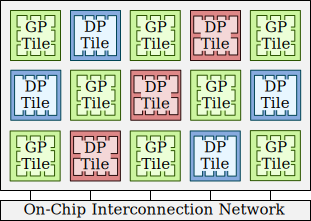
\includegraphics[width=\tw]{intro-overview.svg.pdf}

  \caption{\textbf{Example of Fine-Grain Heterogeneous Architectures --}
    A sea of lightweight compute tiles composed of both general-purpose
    tiles (CPUs) and accelerators specialized for exploiting varying
    forms of parallelism (GPUs for graphics and DSPs for digital signal
    processing).}

  \label{fig-intro-overview}

%\end{figure}

  \end{minipage}%
  \hfill%
  \begin{minipage}[b]{0.56\tw}
    %=========================================================================
% fig-intro-vision
%=========================================================================

%\begin{figure}

  \centering
  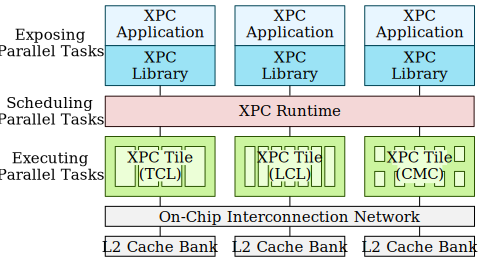
\includegraphics[width=\tw]{intro-vision.svg.pdf}

  \caption{\textbf{XPC Architecture Overview --} XPC applications use an
    XPC parallel programming library to expose fine-grain parallel
    tasks. A software runtime is used to facilitate adaptive task
    distribution to the available hardware resources based on collected
    heuristics. Heterogeneous XPC tiles are specialized for various forms
    of parallelism, but all XPC tiles have the same ISA.}

  \label{fig-intro-vision}

%\end{figure}

  \end{minipage}
\end{figure}

Microprocessor design has reached the limits of improving performance and
energy efficiency by scaling the number of general-purpose cores on a
chip. Instead, computer architects are increasingly using a heterogeneous
mix of general-purpose cores and data-parallel accelerators to exploit
the ubiquitous data parallelism present in modern applications such as
graphics rendering, computer vision, audio processing, graph processing,
physical simulation, big data analytics, and machine learning. Recent
examples include Intel
Haswell~\cite{hammarlund-intel-haswell-ieeemicro2014}, AMD
Kabini~\cite{bouvier-amd-kabini-ieeemicro2014}, and NVIDIA Tegra
4~\cite{krewell-nvidia-tegra4-mpr2013}, which integrate general-purpose
multicores with programmable graphics processing units (GPUs) at a coarse
granularity. While this is a promising first step, coarse-grain
integration makes it difficult to exploit fine-grain parallelism and/or
to rapidly migrate applications between general-purpose processors and
GPUs. \BF{We are interested in exploring future systems that use a
  \emph{fine-grain intermingling} of many lightweight general-purpose
  cores and data-parallel accelerators unified through a common
  instruction set with support for \emph{seamless adaptive execution} of
  parallel tasks as shown in Figure~\ref{fig-intro-overview}.}

Data-parallel accelerators like those used in current coarse-grain
heterogeneous architectures focus on exploiting \emph{conventional data
  parallelism} in which tasks generally have highly regular control and
memory-access structure and do not interact with each other. However,
many applications exhibit \emph{amorphous data parallelism}, a more
general form of data parallelism where tasks are generated dynamically
and can modify the underlying data structures in unpredictable ways
potentially creating inter-task conflicts~\cite{pingali-tao-pldi2011}.
Mapping such applications to current data-parallel accelerators can be
difficult and usually requires aggressive software
optimizations~\cite{luo-gpu-bfs-dac2010,harish-large-graph-gpu-hipc2007,
  hong-cuda-max-warp-ppopp2011,nasre-data-vs-topo-ipdps2013,
  nasre-morph-ppopp2013,mendez-optimizations-amorphous-ppopp2010,
  mendez-gpu-pta-ppopp2012}. Ideally, future fine-grain heterogeneous
architectures would include accelerators suitable for a broad range of
amorphous data parallelism, providing more opportunities for adaptively
scheduling tasks to the best-suited accelerator. These
amorphous-data-parallel accelerators would be specialized not only for
varying degrees of irregularity, but also for efficient dynamic task
generation and conflict resolution.

\BF{This proposal outlines the explicit-parallel-call (XPC) architecture,
  a novel fine-grain heterogeneous architecture based on the concept of
  explicitly encoding parallel tasks as parallel function calls in the
  software/hardware interface.} Figure~\ref{fig-intro-vision} highlights
the vertically integrated approach that will be used to explore software
and hardware techniques for \emph{exposing}, \emph{executing}, and
\emph{scheduling} fine-grain parallel tasks.

